%% Supplementary Information for the Scientific Reports version.
%% Numbers: paper/submission/main.tex. Compile with pdflatex (no bibliography run needed).
\documentclass[10pt,a4paper]{article}
\usepackage[margin=2cm]{geometry}
\usepackage{graphicx}
\usepackage{amsmath,amssymb}
\usepackage{booktabs}
\usepackage{caption}
\usepackage[hidelinks]{hyperref}

\renewcommand{\thefigure}{S\arabic{figure}}
\renewcommand{\thetable}{S\arabic{table}}
\renewcommand{\figurename}{Supplementary Fig.}
\renewcommand{\tablename}{Supplementary Table}
\captionsetup{labelfont=bf, labelsep=period, font=small, justification=raggedright, singlelinecheck=false}
\setlength{\parindent}{0pt}
\emergencystretch=3em
\setlength{\parskip}{4pt}

\newcommand{\tbf}[1]{\textbf{#1}}

\begin{document}

{\large\bfseries Supplementary Information}\par
{\bfseries Observability-gated fusion of sensor measurements and a neural network improves learned visual--inertial odometry}\par
Nada El Madah, Magdy Zakaria, Samir Elmougy, Shahenda Sarhan, Mohamed Handosa and Rasha Elsayed Sakr\par
\medskip

This file contains three supplementary figures (S1--S3) and three supplementary tables (S1--S3) that are cited in the main article. Abbreviations are those of the main article: VIO, visual--inertial odometry; IMU, inertial measurement unit; ATE, absolute trajectory error; $t_\mathrm{rel}$ and $r_\mathrm{rel}$, relative translation and rotation errors.

\section*{Supplementary figures}

\begin{figure}[ht]
\centering
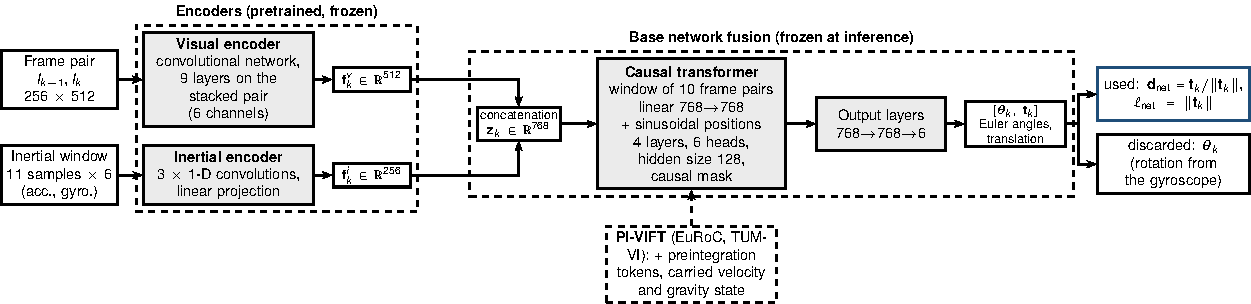
\includegraphics[width=\textwidth]{figures/learned_branch.pdf}
\caption{\tbf{Learned branch.} For each frame pair $k$, frozen VS-VIO encoders map the stacked frame pair and the 11 interpolated IMU samples to a 768-dimensional latent vector; the causal transformer of the base network fuses the last 10 latent vectors and regresses a six-degree-of-freedom relative pose. The gate uses only the translation, split into direction and length; the predicted rotation is discarded in favour of the gyroscope. On EuRoC and TUM-VI we use PI-VIFT (dashed, Supplementary Fig.~S2), whose output layers differ: they output residual corrections. No component is retrained for the gate.}
\end{figure}

\begin{figure}[ht]
\centering
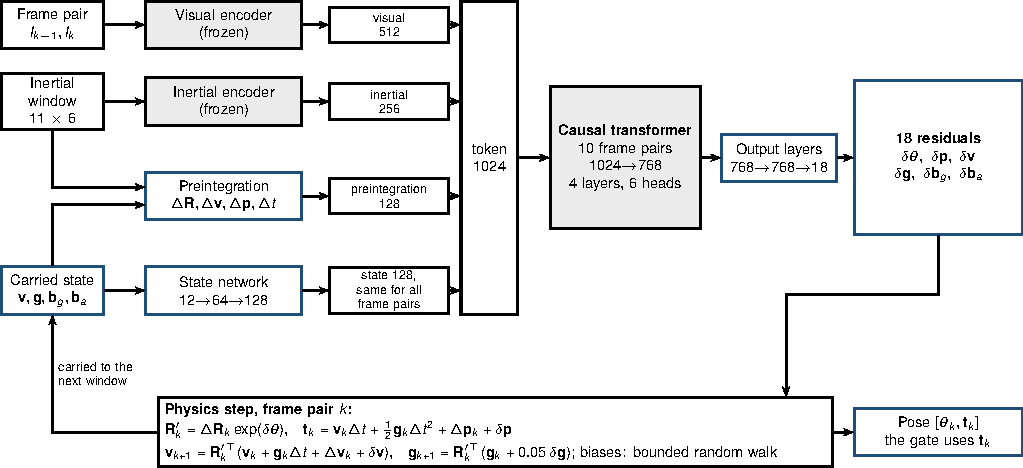
\includegraphics[width=\textwidth]{figures/pivift.pdf}
\caption{\tbf{PI-VIFT.} Blue outlines: what it adds to the base network. Besides the visual and inertial latent vectors, each frame-pair token carries a preintegration token and a state token. The output layers produce 18 residual corrections; the physics step adds them to a kinematic prediction (rotation $\Delta\mathbf R_k$ from the gyroscope, translation from the carried velocity, gravity and the preintegrated acceleration), updates velocity, gravity and biases from one frame pair to the next, and carries the state to the next window. $\Delta\mathbf R_k$, $\Delta\mathbf v_k$ and $\Delta\mathbf p_k$ come from preintegrating the IMU window with the current biases.}
\end{figure}

\begin{figure}[ht]
\centering
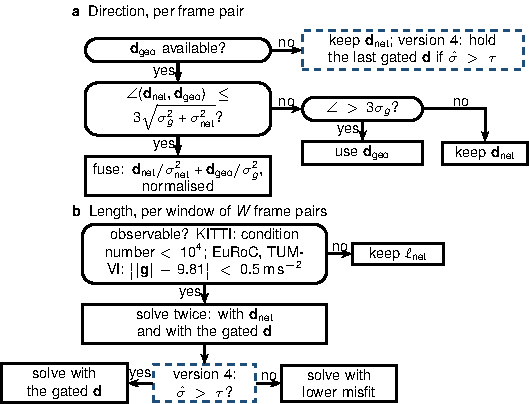
\includegraphics[width=0.8\textwidth]{figures/gate_decisions.pdf}
\caption{\tbf{Gate decisions.} \tbf{a}, Direction: fused where network and geometry agree within their combined uncertainty, geometry where they clearly disagree, network otherwise; without geometry, version 4 holds the last gated direction once the network is distrusted (blue dashed outline). \tbf{b}, Length: the accelerometer where its window is observable, the network elsewhere. Rotation always comes from the gyroscope. Version 3 uses a fixed network direction uncertainty of $0.83^\circ$; version 4 replaces it by the online estimate $\hat\sigma$.}
\end{figure}

\section*{Supplementary tables}

\begin{table}[ht]
\centering
\caption{\tbf{The four gate versions.} KITTI: $t_\mathrm{rel}$ (\%) on the split that includes drive 08, against OXTS; EuRoC: ATE (m) over four sequences, two models; TUM-VI: ATE (m), mean of three seeds. The hand-designed pipelines score 1.27, 1.02 and 0.47 on the three datasets.}
\small
\begin{tabular}{@{}llccc@{}}
\toprule
Version & Status & KITTI & EuRoC & TUM-VI \\
\midrule
v1 & Pre-registered & 1.96 (fail) & 1.01 / 0.98 & Not run \\
v2 & Post-hoc & 1.99 (fail) & 1.00 / 0.96 & Not run \\
v3 & One test run & \tbf{1.21} & 0.94 / 0.99 & 0.69 (fail) \\
v4 & Post-hoc & \tbf{1.21} & 0.95 / 0.98 & \tbf{0.47} \\
\bottomrule
\end{tabular}
\end{table}

\begin{table}[ht]
\centering
\caption{\tbf{Sensitivity to the KITTI condition-number bound} (window of 500 frame pairs). Training: share of frame pairs that use the IMU length and the median relative error of those lengths. Test: $t_\mathrm{rel}$ (\%), mean of three seeds (with 08: split that includes drive 08; no 08: clean split with mirror augmentation).}
\small
\begin{tabular}{@{}lcccc@{}}
\toprule
Bound & Frame pairs using IMU & Length error & With 08 & No 08 \\
\midrule
$10^3$ & 2\% & 5.5\% & 1.61 & 1.96 \\
$\mathbf{10^4}$ (fixed) & 41\% & 1.2\% & 1.27 & 1.55 \\
$10^5$ & 55\% & 1.2\% & 1.27 & 1.55 \\
$10^6$ & 55\% & 1.2\% & 1.27 & 1.55 \\
\bottomrule
\end{tabular}
\end{table}

\begin{table}[ht]
\centering
\caption{\tbf{Comparison with prior work and the change in error.} KITTI drives 05, 07 and 10: $t_\mathrm{rel}$ (\%) / $r_\mathrm{rel}$ ($^\circ$ per 100 m); ours is the gate on the clean split (1.56 / 0.18), or on the split of the released code (1.21 / 0.18) where the prior result uses drive 08. EuRoC and TUM-VI: ATE (m); ours is the gate (0.94 and 0.99 on EuRoC, 0.47 on TUM-VI). Reported numbers are copied from the cited papers and not rerun; ``our runs'' are our reproductions. Negative change: ours is lower. Abs., absolute change.}
\small
\setlength{\tabcolsep}{3pt}
\begin{tabular}{@{}llccc@{}}
\toprule
Prior work & Protocol & Reported & Ours & Change, abs. (\%) \\
\midrule
\multicolumn{5}{@{}l}{\emph{KITTI: $t_\mathrm{rel}$ / $r_\mathrm{rel}$}} \\
VIFT + RPMG [1] & No 08, test-selected & 1.96 / 0.46 & \tbf{1.56 / 0.18} & $-0.40$ ($-20$) / $-0.28$ ($-61$) \\
DB-VIO [2] & Not confirmed & 1.77 / 0.69 & \tbf{1.56 / 0.18} & $-0.21$ ($-12$) / $-0.51$ ($-74$) \\
MixVIO [3] & Abstract only & 1.69 / -- & \tbf{1.56 / 0.18} & $-0.13$ ($-8$) / -- \\
DAP-Pose, camera + IMU [4] & With 08 & 1.90 / 0.54 & \tbf{1.21 / 0.18} & $-0.69$ ($-36$) / $-0.36$ ($-67$) \\
DAP-Pose, + satellite positioning [4] & With 08 & 1.31 / 0.46 & \tbf{1.21 / 0.18} & $-0.10$ ($-8$) / $-0.28$ ($-61$) \\
\midrule
\multicolumn{5}{@{}l}{\emph{EuRoC and TUM-VI: ATE (m)}} \\
Learned base-style, EuRoC & Our runs & 4.02--4.98 & \tbf{0.94--0.99} & $-3.0$ to $-4.0$ ($-75$ to $-81$) \\
Learned networks, TUM-VI & Our runs & 5.0--8.8 & \tbf{0.47} & $-4.5$ to $-8.3$ ($-90$ to $-95$) \\
VINS-Mono [5], EuRoC & Literature & 0.15 & \tbf{0.94} & $+0.79$ (6.3 times higher) \\
ORB-SLAM3, EuRoC & Our runs & 0.042 & \tbf{0.94} & $+0.90$ (22 times higher) \\
\bottomrule
\end{tabular}
\end{table}

\section*{References cited in this file}
\raggedright

\begin{enumerate}
\item Kurt, Y. B., Akman, A. \& Alatan, A. A. Causal transformer for fusion and pose estimation in deep visual inertial odometry. Preprint at \url{https://arxiv.org/abs/2409.08769} (2024).
\item Wan, Z. \& Zhao, L. DB-VIO: dual-branch visual inertial odometry with enhanced visual-inertial representation. Preprint at \url{https://arxiv.org/abs/2607.22123} (2026).
\item Ma, L. \emph{et al.} MixVIO: selective visual-inertial odometry via phase-aware attention and hybrid kernel modeling. \emph{IEEE Robot. Autom. Lett.} \tbf{11}, 9859--9866 (2026).
\item Lin, J. \emph{et al.} DAP-Pose: deep temporal alignment and physics-aware cross-modal sensor fusion for robust pose estimation. Preprint at \url{https://arxiv.org/abs/2607.23755} (2026).
\item Delmerico, J. \& Scaramuzza, D. A benchmark comparison of monocular visual-inertial odometry algorithms for flying robots. In \emph{Proc. IEEE Int. Conf. Robot. Autom. (ICRA)} 2502--2509 (2018).
\end{enumerate}

\end{document}
